\documentclass[10pt]{article}

\usepackage[utf8]{inputenc}
\usepackage[T1]{fontenc}
\usepackage{lmodern}
\usepackage[margin=0.78in]{geometry}
\usepackage{amsmath,amssymb,mathtools}
\usepackage{array,booktabs,graphicx}
\usepackage{hyperref}
\usepackage{xcolor}

\hypersetup{
  colorlinks=true,
  linkcolor=blue!55!black,
  citecolor=blue!55!black,
  urlcolor=blue!55!black
}
\setlength{\emergencystretch}{2em}

\title{\textbf{Exact High-Dimensional Ehrhart Polynomials and Volumes of Bounded-Treewidth Order Polytopes via Nice Tree Decompositions and CRT}}
\author{Wendel León Alvarado}
\date{November 12, 2026}

\begin{document}
\maketitle

\begin{abstract}
We present an exact modular dynamic program for Ehrhart data of order polytopes whose Hasse graphs have small treewidth. A minimum-fill elimination heuristic produces a tree decomposition, which is converted to a nice decomposition with leaf, introduce, forget, and join nodes. Each boundary table is a tensor over a finite chain. At a forget node, all constraints incident to the eliminated element reduce its admissible coordinate to an interval; an axis-wise modular prefix sum contracts that coordinate. Join nodes combine independent subproblems by a Hadamard product. Counts are reconstructed without integer overflow using 61-bit primes and a bound of $(m+1)^d$ on the number of lattice points in the $m$th dilation. The resulting exact Ehrhart polynomial yields the normalized volume and the rational Euclidean volume. Experiments on 12 instances from cyclic crowns, layered residual DAGs, and series-parallel posets reach dimension $d=40$. A layered DAG with measured treewidth two has normalized volume $1{,}423{,}698{,}065{,}794{,}236{,}220{,}560$, while the largest measured peak traced memory in the benchmark is 238.4 MB for the dimension-16 treewidth-four crown.
\end{abstract}

\noindent\textbf{Keywords:} order polytope; Ehrhart polynomial; treewidth; nice tree decomposition; tensor contraction; Chinese remainder theorem; exact volume.

\section{Introduction}

For a finite poset $P=(V,\preceq)$ with $d=|V|$, its order polytope is
\[
\mathcal{O}(P)=\{x\in[0,1]^V:x_u\leq x_v\text{ whenever }u\preceq v\}.
\]
The inequalities on cover relations suffice. This class includes cyclic crown posets, periodic stencil dependencies, distributed ring-buffer precedence constraints, and irregular DAG precedence systems. It also provides a combinatorial model for monotone regions arising in piecewise-linear network analysis and for constrained latent-variable configurations. The applications motivate the model; the computations below concern the exact order-polytope problem and do not claim empirical performance on those application domains.

The order polytope has an integral, unimodular triangulation indexed by linear extensions of $P$. Consequently its normalized volume is an integer and equals the number of linear extensions. In high dimension, however, explicit triangulation can be infeasible even when the Hasse graph is sparse. This paper uses treewidth as the structural parameter and avoids enumerating simplices.

For an integer $m\geq0$, define
\[
L_P(m)=\#\bigl(m\mathcal{O}(P)\cap\mathbb{Z}^d\bigr)
=\#\{x:V\to\{0,\ldots,m\}:x_u\leq x_v\text{ for every cover }u\lessdot v\}.
\]
The Ehrhart series and $h^*$-polynomial satisfy
\[
\sum_{m\geq0}L_P(m)z^m=\frac{h_P^*(z)}{(1-z)^{d+1}},
\qquad
h_i^*=\sum_{j=0}^{i}(-1)^{i-j}\binom{d+1}{i-j}L_P(j).
\]
In particular,
\[
H_P(1):=h_P^*(1)=d!\operatorname{Vol}(\mathcal{O}(P)).
\]
Since each of the $d$ coordinates has $m+1$ possible values,
\[
0\leq L_P(m)\leq(m+1)^d\leq(d+1)^d,\qquad 0\leq m\leq d.
\]
This elementary bound is sufficient for deterministic Chinese-remainder reconstruction.

\paragraph{Contributions.}
We give an implementable nice-tree-decomposition dynamic program with modular tensors; reconstruct $L_P(0),\ldots,L_P(d)$ and the complete $h^*$-vector exactly; and report a multi-family benchmark through $d=40$, including exact agreement with two independent cyclic-crown reference vectors.

\section{Algorithmic Framework}

\subsection{Minimum-fill decomposition and boundary states}

We form the undirected Hasse graph and run deterministic minimum-fill elimination, breaking ties by current degree and then by vertex label. Eliminating a vertex creates a bag containing that vertex and its remaining neighbors; fill edges make the bag a clique. The elimination bags define a tree decomposition of width at most the largest bag size minus one. We convert the decomposition to a rooted nice form with \textsc{Leaf}, \textsc{Introduce}, \textsc{Forget}, and binary \textsc{Join} nodes. The reported width is the width found by this heuristic, not a certificate that the graph's optimal treewidth has been found.

For a fixed dilation $m$, write $q=m+1$ and let a bag be $B$. The dynamic-programming tensor is indexed by boundary assignments $a:B\to\{0,\ldots,m\}$; its entry counts compatible assignments in the processed part of the decomposition, modulo a prime $p$. A bag of size $b$ therefore has $q^b$ entries.

\subsection{Nice-node operators}

\begin{itemize}
\item \textsc{Leaf}: return the scalar tensor $1$ on the empty bag.
\item \textsc{Introduce}$(v)$: insert a new axis of length $q$ by broadcasting the child tensor. This creates the boundary coordinate for $v$; it does not prematurely sum over that coordinate.
\item \textsc{Forget}$(v)$: for a fixed assignment to the parent bag, the cover relations incident to $v$ restrict $x_v$ to
\[
\ell(a)=\max\bigl(\{0\}\cup\{a(u):u\lessdot v,\ u\in B\}\bigr),
\quad
u(a)=\min\bigl(\{m\}\cup\{a(w):v\lessdot w,\ w\in B\}\bigr).
\]
The forgotten axis is contracted over $\ell(a)\leq x_v\leq u(a)$. An axis-wise prefix sum computes each interval sum by two modular table lookups; empty intervals contribute zero. This applies the order masks exactly once when the variable is eliminated.
\item \textsc{Join}: multiply the two child tensors entrywise modulo $p$. The two subproblems share only their boundary assignment, so the product combines their independent interior choices.
\end{itemize}

The prefix transform belongs at \textsc{Forget}, where the coordinate being summed out is available as an axis. Applying this contraction at \textsc{Introduce} would discard a boundary value that must still be passed to the parent. Thus the implementation uses a neutral axis expansion at introduce nodes and performs the fast prefix/suffix interval contraction at forget nodes.

Every tensor entry is reduced modulo $p$. The implementation uses exact 61-bit primes and a specialized modular product for join tensors; no floating-point arithmetic enters the count.

\subsection{CRT reconstruction and Ehrhart extraction}

For each $m=0,\ldots,d$, the point count is computed modulo a set of distinct 61-bit primes whose product exceeds
\[
M_d=(d+1)^d.
\]
The exact bound is valid for every required dilation. Therefore the Chinese-remainder representative in $[0,\prod p_i)$ is the unique integer $L_P(m)$, not merely a residue or an estimate. Substitution into the binomial transform above gives every coefficient of $h_P^*(z)$; summing the coefficients gives $H_P(1)$, and division by $d!$ gives the reduced rational Euclidean volume.

\section{Parameterized Complexity and Space}

Let $\tau$ be the width of the decomposition returned by the heuristic, and let $r$ be the number of primes. For a single dilation $m$ and one prime, each table has at most $(m+1)^{\tau+1}$ entries. A nice decomposition has $O(d(\tau+1))$ transition work under the standard bag-difference construction; an axis prefix contraction costs $O((\tau+1)(m+1)^{\tau+1})$ in the direct implementation. Thus the modular computation for one dilation over all CRT primes is bounded by
\[
O\!\left(d(\tau+1)(m+1)^{\tau+1}r\right)
=O\!\left(d(\tau+1)(m+1)^{\tau+1}\log M_d\right),
\]
where the 61-bit prime size is a fixed constant. This is the per-dilation bound. Recovering the full Ehrhart vector requires all $d+1$ dilations; summing the per-dilation costs gives
\[
O\!\left(d(\tau+1)\log M_d\sum_{m=0}^{d}(m+1)^{\tau+1}\right)
=O\!\left(d(\tau+1)(d+1)^{\tau+2}\log M_d\right).
\]
The sum accounts for all dilation alphabets. In particular, the often-quoted $O(d\,\tau\,(d+1)^{\tau+1}\log M_d)$ form describes a single largest-alphabet pass, not all $d+1$ dilation passes performed here.

The state space of one bag table is $O((m+1)^{\tau+1})$, and the largest table payload over the required dilations is $O((d+1)^{\tau+1})$. The implementation evaluates the decomposition recursively and materializes join operands and prefix-sum temporaries; consequently its measured process-level traced peak also includes simultaneously live intermediate arrays and is not asserted to equal the single-table payload bound. This distinction is visible in the treewidth-four instance below. The advantage is structural: the tensor dimension depends exponentially on treewidth, rather than on the number of linear extensions or the total number of simplices.

\section{Multi-Family Benchmark through Dimension 40}

All reported instances were processed exactly. The families comprise two cyclic crowns, six layered DAGs with local and residual connections, and four sparse series-parallel posets. The two crowns have exact agreement with the stored reference $h^*$-vectors, normalized volumes, and Euclidean volumes. For example,
\[
h_{C_{3,4}}^*=(1,69,1204,7164,16906,16906,7164,1204,69,1),
\quad H_{C_{3,4}}(1)=50{,}688,
\]
and $50{,}688/12!=1/9450$. For $C_{4,4}$, the exact normalized volume is $2{,}363{,}392$ and its Euclidean volume is $577/5{,}108{,}103{,}000$. The full coefficient vectors, point counts, CRT primes, and reduced rational volumes for every instance are included in \texttt{resultados\_treewidth\_crt.json}.

\begin{table}[htbp]
\centering
\caption{Complete benchmark inventory and measured exact-computation metrics. Time is wall-clock seconds; memory is Python \texttt{tracemalloc} peak in MB; $r$ is the number of CRT primes. The exact Euclidean volume is $H_P(1)/d!$.}
\label{tab:benchmark}
\scriptsize
\setlength{\tabcolsep}{3.2pt}
\resizebox{\textwidth}{!}{%
\begin{tabular}{llrrrrrr}
\toprule
Family & Instance & $d$ & $\tau$ & $r$ & Time (s) & Peak (MB) & $H_P(1)$\\
\midrule
Crown & $C_{3,4}$ & 12 & 2 & 1 & 0.173327 & 0.376603 & 50,688\\
Crown & $C_{4,4}$ & 16 & 4 & 2 & 14.011996 & 238.401336 & 2,363,392\\
Layered DAG & $w=3,\ell=5$ & 15 & 2 & 1 & 0.212862 & 0.679631 & 428,934\\
Layered DAG & $w=4,\ell=5$ & 20 & 2 & 2 & 0.685400 & 1.535143 & 6,650,192,736\\
Layered DAG & $w=3,\ell=8$ & 24 & 2 & 2 & 1.462309 & 3.039813 & 3,293,875,020\\
Layered DAG & $w=3,\ell=10$ & 30 & 2 & 3 & 3.997101 & 5.751975 & 1,679,561,591,895\\
Layered DAG & $w=4,\ell=9$ & 36 & 2 & 4 & 9.300289 & 9.788984 & 6,826,310,903,479,957,120\\
Layered DAG & $w=4,\ell=10$ & 40 & 2 & 4 & 12.057713 & 13.233064 & 1,423,698,065,794,236,220,560\\
Series-parallel & $d=18$ & 18 & 2 & 2 & 0.508418 & 0.163203 & 32\\
Series-parallel & $d=25$ & 25 & 2 & 2 & 1.047872 & 0.355191 & 256\\
Series-parallel & $d=32$ & 32 & 2 & 3 & 3.202047 & 0.689274 & 1,024\\
Series-parallel & $d=40$ & 40 & 2 & 4 & 7.653119 & 1.241556 & 8,192\\
\bottomrule
\end{tabular}}
\end{table}

Figure~\ref{fig:scaling} compares measured wall time and peak traced memory by family and reported width. The only width-four benchmark is $C_{4,4}$; its memory peak also includes temporary arrays and is not representative of the width-two DAG runs. The dashed 15-second line records the historical timeout threshold from dimension-matched $C_{k,5}$ triangulation references. Those references are different posets, so the line is contextual and is not presented as a same-instance speedup comparison.

\begin{figure}[htbp]
\centering
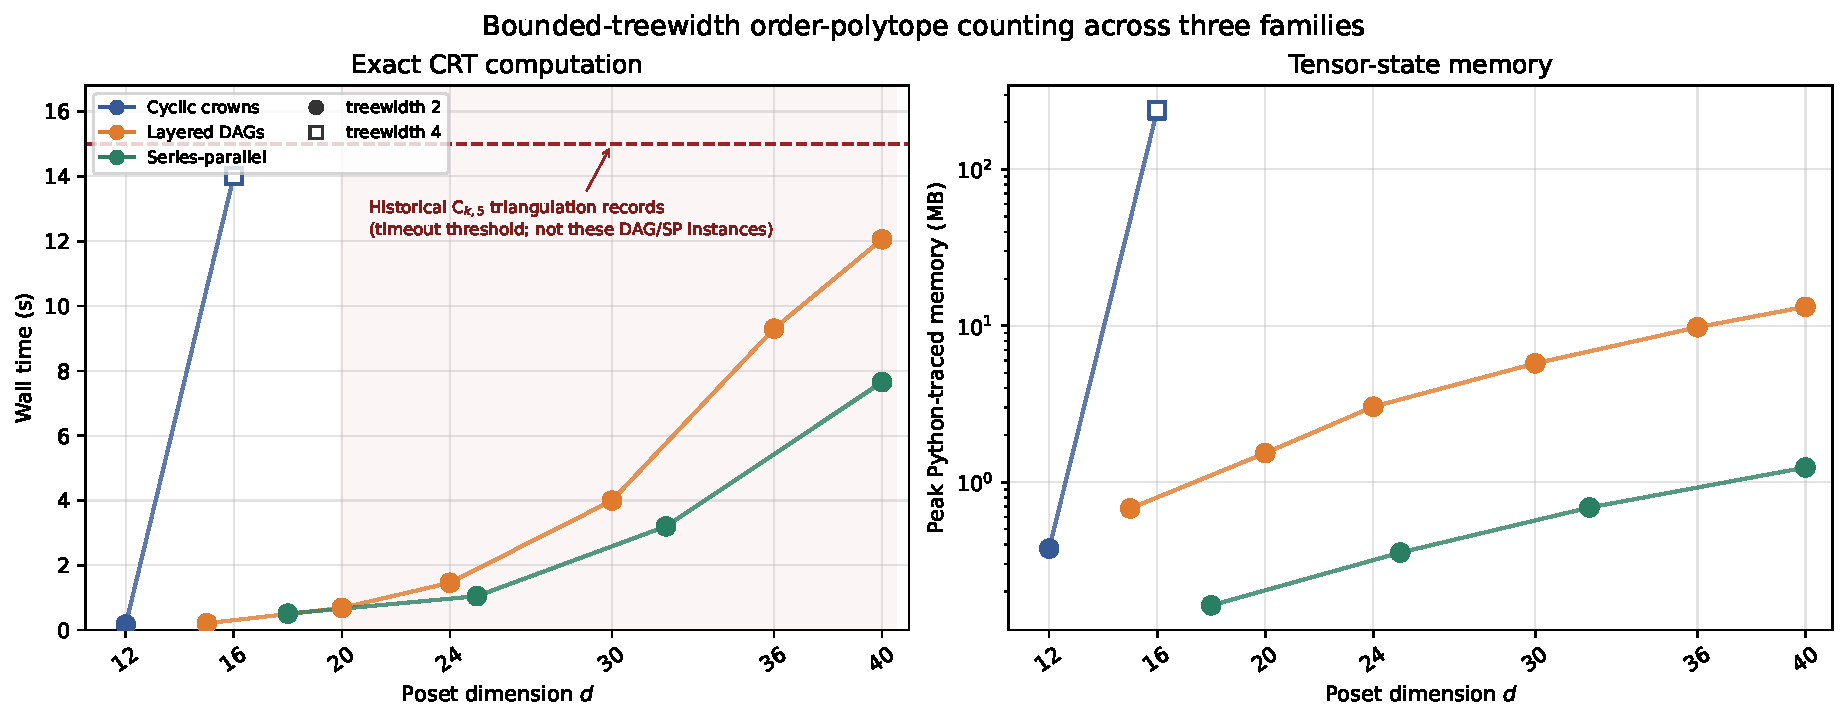
\includegraphics[width=\textwidth]{fig_treewidth_scaling.pdf}
\caption{Runtime and memory across the 12 instances. Filled circles mark reported width two; the open square marks width four. The historical timeout threshold is explicitly contextual.}
\label{fig:scaling}
\end{figure}

Figure~\ref{fig:dagvol} separates the exact normalized volume from the measured tensor-DP memory for the six layered DAGs. Their $h^*$-vectors and volumes were reconstructed over the integers, including the $d=40$ value above $10^{21}$.

\begin{figure}[htbp]
\centering
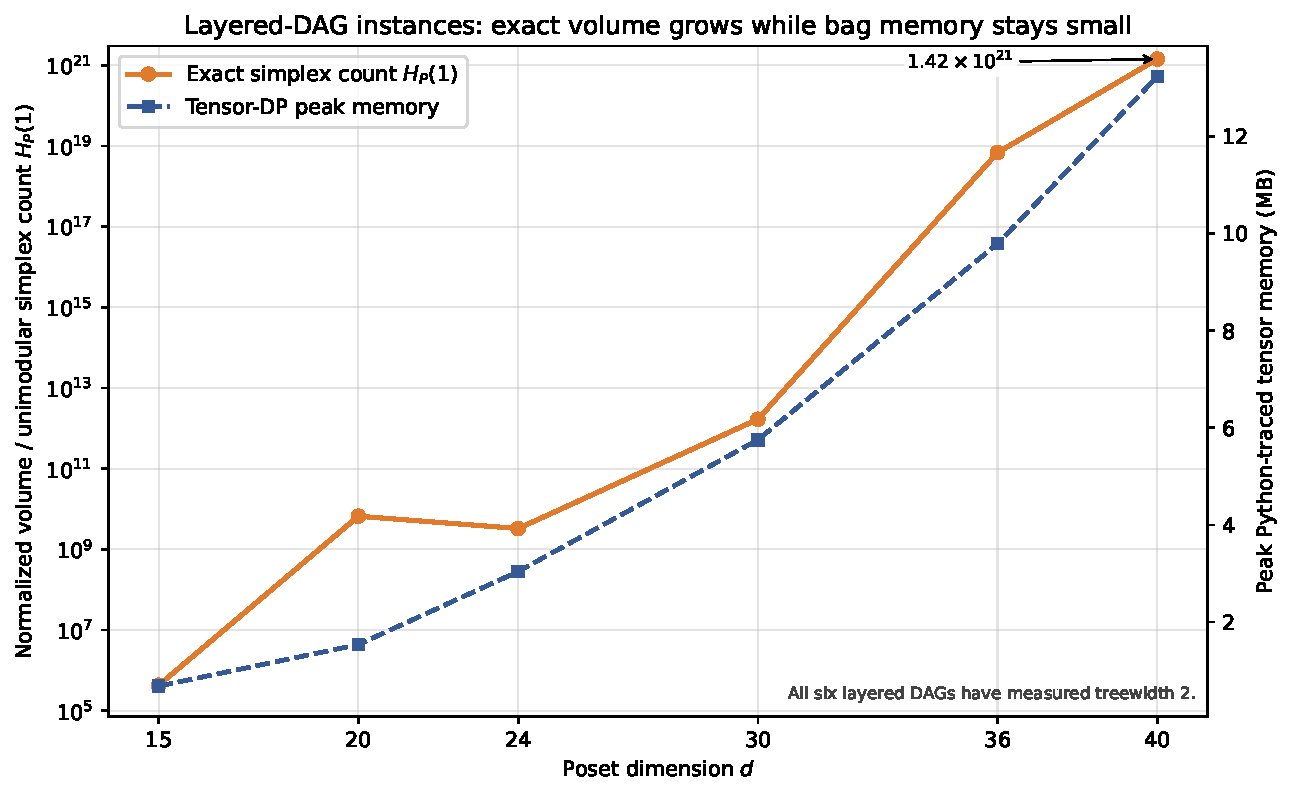
\includegraphics[width=0.88\textwidth]{fig_dag_volumes_d40.pdf}
\caption{Exact normalized volume $H_P(1)$ (log scale) and peak traced memory for layered DAGs of measured treewidth two.}
\label{fig:dagvol}
\end{figure}

\subsection{Exact validation and interpretation}

For the two crown instances, the independently stored benchmark vectors match coefficient by coefficient; their normalized and Euclidean volumes also match exactly. The exact brute-force checks in the implementation cover small posets and dilations. These validations test the modular transfer, the CRT reconstruction, and the Ehrhart binomial transform through independent routes.

The 15-second historical cutoff should not be read as a direct comparison for every row in Table~\ref{tab:benchmark}. The recorded triangulation baseline is a contextual, dimension-matched $C_{k,5}$ reference, not a rerun on each DAG or series-parallel instance. In particular, the larger observed crown time at $C_{4,4}$ is an actual run of the present method and is reported without extrapolating from the historical threshold.

\section{Conclusion and Reproducibility}

Nice tree decompositions turn exact order-polytope counting into modular tensor operations whose table size is governed by bag width. A simple coordinate bound supplies enough CRT primes for exact reconstruction of every point count needed for the $h^*$-polynomial, normalized volume, and rational Euclidean volume. The 12-instance benchmark reaches dimension 40 and demonstrates that very large exact volumes can coexist with modest memory on width-two instances.

The complete implementation, input constructions, raw exact outputs, and figure generator are in \path{TREEWIDTH_TENSOR_CRT/}. Reproduce the figures with
\begin{quote}
\small\ttfamily
.venv\textbackslash Scripts\textbackslash python.exe\\
TREEWIDTH\_TENSOR\_CRT\textbackslash generar\_graficas\_treewidth.py
\end{quote}
The same decomposition framework may be extended to sparse rational systems $Ax\leq b$ when their local constraints admit finite-state boundary tables; such extensions require suitable exact discretization or weighted state representations and are left for future work.

\begin{thebibliography}{9}
\bibitem{Stanley1986}
R. P. Stanley,
\newblock Two poset polytopes,
\newblock \emph{Discrete \& Computational Geometry}, 1 (1986), pp. 9--23.

\bibitem{Bodlaender1996}
H. L. Bodlaender,
\newblock A linear-time algorithm for finding tree-decompositions of small treewidth,
\newblock \emph{SIAM Journal on Computing}, 25 (1996), no. 6, pp. 1305--1317.
\end{thebibliography}

\end{document}
